%%%%%%%%%%%%%%%%%%%%%%%%%%%%%%%%%%%%%%%%%
% Short Sectioned Assignment LaTeX Template Version 1.0 (5/5/12)
% This template has been downloaded from: http://www.LaTeXTemplates.com
% Original author:  Frits Wenneker (http://www.howtotex.com)
% License: CC BY-NC-SA 3.0 (http://creativecommons.org/licenses/by-nc-sa/3.0/)
%%%%%%%%%%%%%%%%%%%%%%%%%%%%%%%%%%%%%%%%%

%----------------------------------------------------------------------------------------
%	PACKAGES AND OTHER DOCUMENT CONFIGURATIONS
%----------------------------------------------------------------------------------------

\documentclass[paper=a4, fontsize=11pt]{scrartcl} % A4 paper and 11pt font size

% ---- Entrada y salida de texto -----

\usepackage[T1]{fontenc} % Use 8-bit encoding that has 256 glyphs
\usepackage[utf8]{inputenc}
%\usepackage{fourier} % Use the Adobe Utopia font for the document - comment this line to return to the LaTeX default

% ---- Idioma --------

\usepackage[spanish, es-tabla]{babel} % Selecciona el español para palabras introducidas automáticamente, p.ej. "septiembre" en la fecha y especifica que se use la palabra Tabla en vez de Cuadro

% NOTA: en caso de problema al compilar, compruebe que tiene el paquete: texlive-babel-spanish.noarch

% ---- Otros paquetes ----

\usepackage{amsmath,amsfonts,amsthm} % Math packages
\usepackage{graphics,graphicx,floatrow} %para incluir imágenes y notas en las imágenes
\usepackage{listings}

\usepackage{url}

%% Define a new 'leo' style for the package that will use a smaller font.
\makeatletter
\def\url@leostyle{%
	\@ifundefined{selectfont}{\def\UrlFont{\sf}}{\def\UrlFont{\small\ttfamily}}}
\makeatother
%% Now actually use the newly defined style.
\urlstyle{leo}
\setlength{\parindent}{12pt}

% Para hacer tablas comlejas
\usepackage{multirow}
\usepackage{threeparttable}

%\usepackage{sectsty} % Allows customizing section commands
%\allsectionsfont{\centering \normalfont\scshape} % Make all sections centered, the default font and small caps

\usepackage{fancyhdr} % Custom headers and footers
\pagestyle{fancyplain} % Makes all pages in the document conform to the custom headers and footers
\fancyhead{} % No page header - if you want one, create it in the same way as the footers below
\fancyfoot[L]{} % Empty left footer
\fancyfoot[C]{} % Empty center footer
\fancyfoot[R]{\thepage} % Page numbering for right footer
\renewcommand{\headrulewidth}{0pt} % Remove header underlines
\renewcommand{\footrulewidth}{0pt} % Remove footer underlines
\setlength{\headheight}{13.6pt} % Customize the height of the header

\numberwithin{equation}{section} % Number equations within sections (i.e. 1.1, 1.2, 2.1, 2.2 instead of 1, 2, 3, 4)
\numberwithin{figure}{section} % Number figures within sections (i.e. 1.1, 1.2, 2.1, 2.2 instead of 1, 2, 3, 4)
\numberwithin{table}{section} % Number tables within sections (i.e. 1.1, 1.2, 2.1, 2.2 instead of 1, 2, 3, 4)

\setlength\parindent{0pt} % Removes all indentation from paragraphs - comment this line for an assignment with lots of text

\newcommand{\horrule}[1]{\rule{\linewidth}{#1}} % Create horizontal rule command with 1 argument of height



\usepackage[utf8]{inputenc}
\usepackage[T1]{fontenc}
\usepackage[spanish]{babel}
\usepackage{times}

\usepackage{color}
\definecolor{gray97}{gray}{.97}
\definecolor{gray75}{gray}{.75}
\definecolor{gray45}{gray}{.45}

\usepackage{listings}
\lstset{ frame=Ltb,
	framerule=0pt,
	aboveskip=0.5cm,
	framextopmargin=3pt,
	framexbottommargin=3pt,
	framexleftmargin=0.4cm,
	framesep=0pt,
	rulesep=.4pt,
	backgroundcolor=\color{gray97},
	rulesepcolor=\color{black},
	%
	stringstyle=\ttfamily,
	showstringspaces = false,
	basicstyle=\small\ttfamily,
	commentstyle=\color{gray45},
	keywordstyle=\bfseries,
	%
	numbers=left,
	numbersep=15pt,
	numberstyle=\tiny,
	numberfirstline = false,
	breaklines=true,
}

% minimizar fragmentado de listados
\lstnewenvironment{listing}[1][]
{\lstset{#1}\pagebreak[0]}{\pagebreak[0]}

\lstdefinestyle{consola}
{basicstyle=\scriptsize\bf\ttfamily,
	backgroundcolor=\color{gray75},
}

\lstdefinestyle{C}
{language=C,
}


\usepackage[pdftex,colorlinks=true,linkcolor=negro,urlcolor=blue]{hyperref,xcolor}
\definecolor{negro}{rgb}{0,0,0}

\graphicspath{ {./imagenes/} }
\usepackage{subfig}
\hypersetup{citecolor=blue}

\title{	
\normalfont \normalsize 
\textsc{{\bf Ingeniería de Servidores (2014-2015)} \\ Grado en Ingeniería Informática \\ Universidad de Granada} \\ [25pt]
\horrule{0.5pt} \\[0.4cm] % Thin top horizontal rule
\huge Memoria Práctica 5 \\ % The assignment title
\horrule{2pt} \\[0.5cm] % Thick bottom horizontal rule
}

\author{Jose Antonio Jiménez Montañés}

\date{\normalsize\today}

%----------------------------------------------------------------------------------------
% DOCUMENTO
%----------------------------------------------------------------------------------------
%
%\begin{figure}[H]
%	\centering
%	\includegraphics[width=0.5\textwidth]{gull}
%	\caption{Texto Prueba}
%	\label{fig:ddd}
%\end{figure}


%\cite{p1}


\begin{document}

\maketitle % Muestra el Título

\newpage %inserta un salto de página

\tableofcontents % para generar el índice de contenidos
\clearpage
\listoffigures

%\listoftables 

\newpage

%----------------------------------------------------------------------------------------
%	Cuestion 1
%----------------------------------------------------------------------------------------
\section{Al modificar los valores del kernel de este modo, no logramos que persistan después de reiniciar la máquina. ¿Qué archivo hay que editar para que los cambios sean permanentes?}

El archivo “/etc/sysctl.conf”.\\
Solamente tenemos que añadir aquella modificación de la variable que queramos que no se pierda al reiniciar el sistema.\\

Si únicamente lo añadimos al fichero de configuración y no ejecutamos sysctl tenemos que actualizar la configuración con sysctl -p para que los cambios sean efectivos al instante.\\


%------------------------------------------------
% CUESTION 2
%------------------------------------------------
\section{Con qué opción se muestran todos los parámetros modificables en tiempo de ejecución? Elija	dos parámetros y explique, en dos líneas, qué función tienen.}

Con la opción “-a” o “-A”. Ésta última nos las muestra en forma de tabla.\\
Parámetro 1:\\
-overcommit\_memory: flag que activa el exceso de memoria.\\
Cuando es 0, el kernel intenta estimar la cantidad memoria libre restante cuando el usuario solicita más memoria.\\
Cuando es 1, el kernel simula tener siempre suficiente memoria hasta que se acaba.\\
Cuando es 2, el kernel usa una política de "nunca overcommit" que intenta evitar cualquier sobre asignación de memoria.\\

Parámetro 2:\\
-file-max: especifica el nº máximo de archivos que el kernel de Linux asignará. Si recibimos mensajes de error sobre la ejecución de estos archivos, deberíamos ampliar el tamaño.\\

\clearpage
%-------------------------------------------------------------------------------------------
% CUESTION 3
%--------------------------------------------------------------------------------------------
\section{Realice una copia de seguridad del registro y restáurela, ilustre el proceso con capturas.}

Hay muchas formas de realizar una copia de seguridad del registro, la que siempre he usado yo es aquella que no exporta los registros sino que copia literalmente los archivos de registro y sustituirlos para restaurar la copia de seguridad.\\

Estos archivos se guardan en el directorio system32/config del directorio de instalación de Windows.\\

El registro está subdividido por secciones y cada sección se almacena en un archivo diferente, por ello es por lo que me inclino por este método ya que en caso de un desastre del sistema por ejemplo a la hora de haber instalado algún driver defectuoso, solo tendremos que restaurar la parte que almacena esta información, lo mismo para problemas de software o problemas de cuentas de usuario.\\

Los archivos que hay que hacerle una copia son:\\
COMPONENTS, DEFAULT, DRIVERS, SAM, SECURITY, SOFTWARE, SYSTEM\\

\begin{figure}[H]
	\centering
	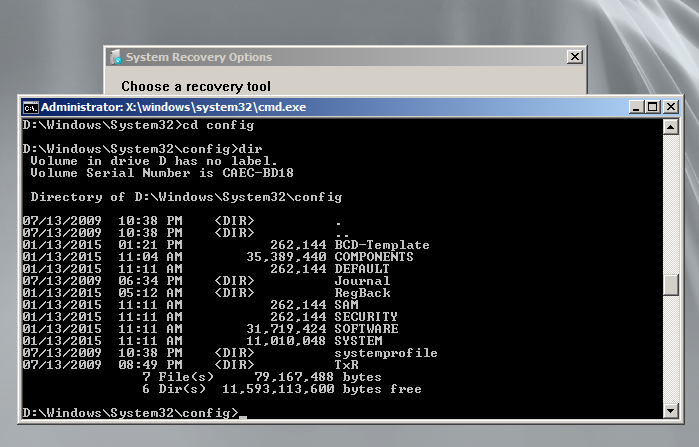
\includegraphics[width=1\textwidth]{c03f01}
	\caption{Contenido del directorio donde se almacena el registro de Windows.}
	\label{fig:c03f01}
\end{figure}
\clearpage
Para restaurar solo bastaría con eliminar los archivos actuales que queramos restaurar y sustituirlos por los de la copia de seguridad.\\

Este proceso ademas puede ser incluso más rápido si nos creamos un archivo batch que nos automatice el proceso.\\

\begin{figure}[H]
	\centering
	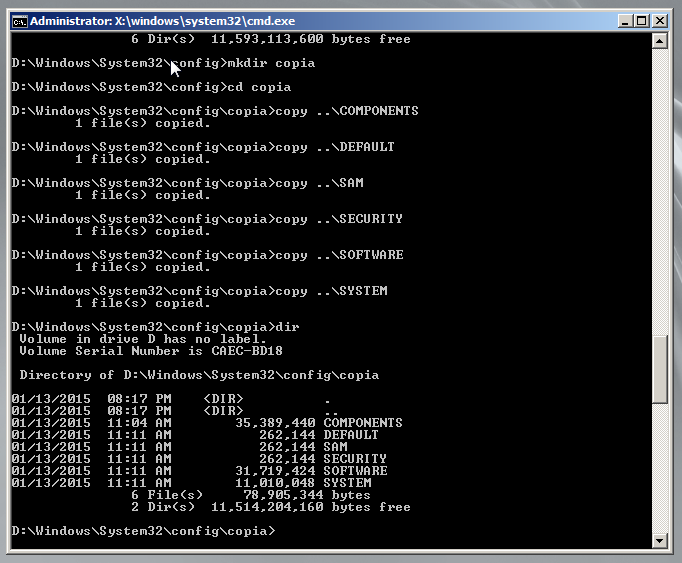
\includegraphics[width=1\textwidth]{c03f03}
	\caption{Realizando copia de seguridad desde la consola de Recuperación.}
	\label{fig:c03f03}
\end{figure}
\clearpage
NOTA: Es importante indicar que tanto para copiar los archivos como para restaurarlos se debe de hacer bajo la consola de recuperación del sistema que siempre estará disponible en el CD o DVD de instalación del mismo, aunque existe un método para instalar dicha consola en el arranque de Windows como una parte aislada del sistema. Si se intenta desde dentro del propio sistema no nos dejará debido a que el registro estará en uso y por tanto protegido.

\begin{figure}[H]
	\centering
	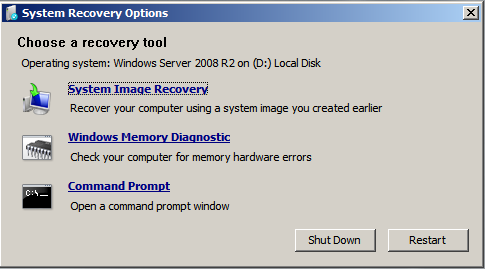
\includegraphics[width=1\textwidth]{c03f02}
	\caption{Menu desde donde se accede a la consola de recuperación de Windows.}
	\label{fig:c03f02}
\end{figure}
\clearpage
%----------------------------------------------------------------------------------------
% CUESTION 4
%----------------------------------------------------------------------------------------
\section{¿Cómo se abre una consola en Windows? ¿Qué comando hay que ejecutar para editar el registro? Muestre su ejecución con capturas de pantalla}

a) O buscamos el acceso directo de "simbolo de sistema", o más rápido ejecutamos el comando "cmd".\\

\begin{figure}[H]
	\centering
	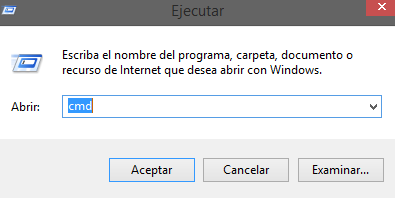
\includegraphics[width=1\textwidth]{c04f01}
	\caption{Ejecucion del simbolo de sistema.}
	\label{fig:c04f01}
\end{figure}

b) Para editarlo de una manera gráfica e intuitiva se usa el comando regedit. Se nos abrirá una aplicación en la cual podemos modificar, buscar, insertar valores y hacer copias de registro así como importar archivos de registro.\\

\begin{figure}[H]
	\centering
	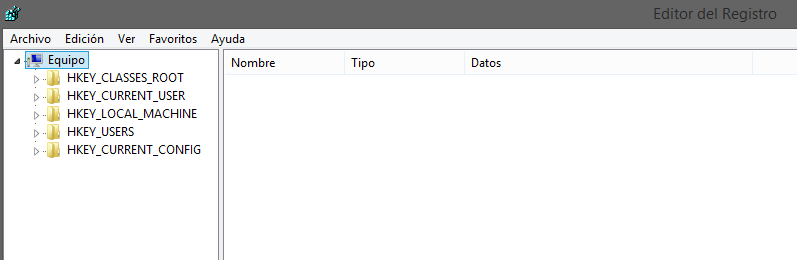
\includegraphics[width=1\textwidth]{c04f02}
	\caption{Ejecucion de regedit.}
	\label{fig:c04f02}
\end{figure}

Otra opción menos visual es mediante consola con el comando "reg" que tiene también la opción de poder agregar, eliminar o realizar copias de seguridad entre otras funciones (Aunque no la de buscar).\\

\begin{figure}[H]
	\centering
	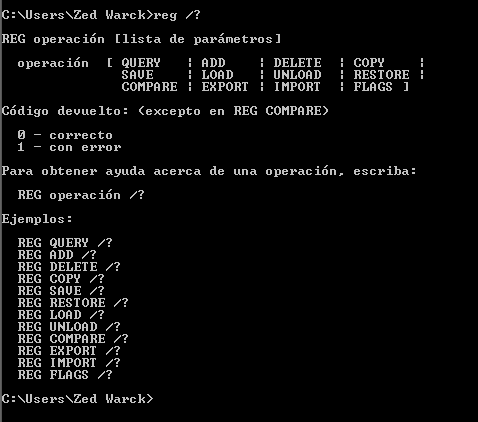
\includegraphics[width=1\textwidth]{c04f03}
	\caption{Ejecucion del comando reg.}
	\label{fig:c04f03}
\end{figure}

\clearpage
%----------------------------------------------------------------------------------------
% CUESTION 5
%----------------------------------------------------------------------------------------
\section{Las cadenas de caracteres y valores numéricos tienen distintos	tipos. Busque en la documentación de Microsoft y liste todos los tipos de valores. \cite{c05c01}}

\begin{figure}[H]
	\centering
	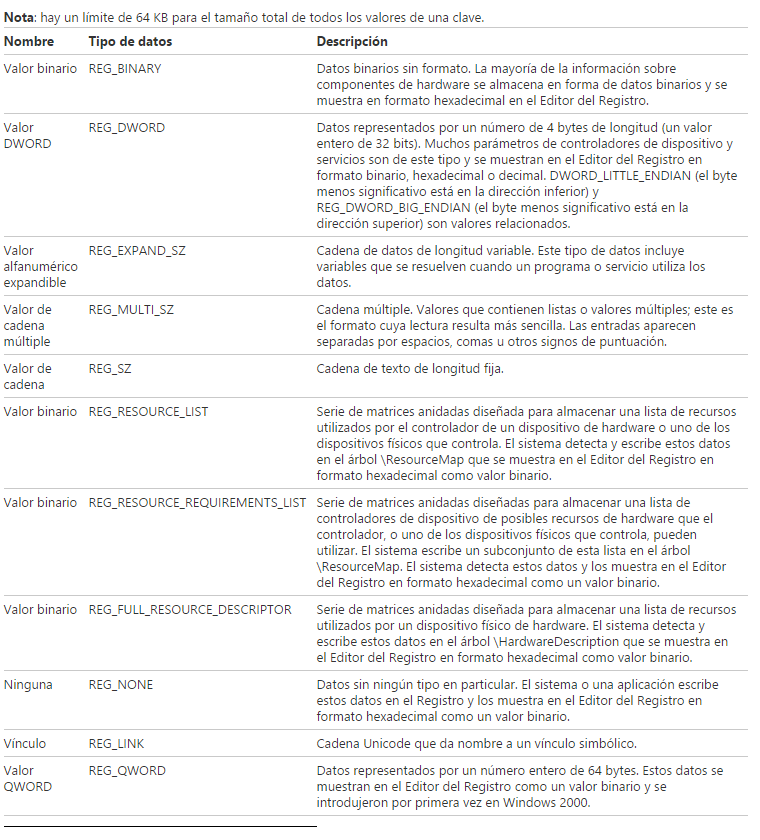
\includegraphics[width=1\textwidth]{c05f01}
	\caption{Posibles valores en el registro de windows.}
	\label{fig:c05f01}
\end{figure}


%----------------------------------------------------------------------------------------
% CUESTION 6
%----------------------------------------------------------------------------------------
\section{Enumere qué elementos se pueden configurar en Apache y en IIS para que Moodle funcione mejor. \cite{c06c01}}

Configuración en APACHE:\\
-Fijar "MaxClients" utilizando la siguiente fórmula:\\
MaxClients= Memoria total disponible*80\\
-Uso máximo de la memoria por el proceso Apache\\
-Si necesitamos incrementar el valor de "MaxClients" por encima de 256, necesitaremos también fijar el parámetro "ServerLimit".\\
-Debemos considerar reducir el nº de módulos que Apache carga en su fichero de configuración (httpd.conf), al mínimo necesario.\\
-En sistemas Unix/Linux hay que disminuir el "MaxRequestPerChild" a unos valores de entre 20 y 30.\\
-Para servidores que vayan a tener un nivel de carga bastante alto debemos poner el parámetro "KeepAlive" en 'off', o bien, disminuir el timeout ("KeepAliveTimeout") a valores entre 2 y 5 (el valor por defecto es 15 segundos).\\
-Si no estamos realizando trabajos de investigaciones con el servidor, estableceremos el ExtendedStatus a 'off'.\\
-Reduciremos el valor del "TimeOut" a unos valores entre 30 y 60 segundos.\\
\\
Configuración en ISS:\\
Todos los cambios a realizar se harán sobre la ubicación del registro:\\
HKLM/SYSTEM/CurrentControlSet/Services/Inetinfo/Parameters/ \\
-Fijaremos el "ListenBackLog" (equivalente a "KeepAliveTimeOut") a unos valores entre 2 y 5.\\
-Cambiaremos el valor de "MemCacheSize" para ajustar la cantidad de memoria en Mb que ISS utilizará para su caché (por defecto se encuentra al 50\%).\\
-Cambiaremos también el valor de "MaxCacheFileSize" para ajustar el tamaño máximo (en bytes) de un archivo que pueda encontrarse en la caché. Por defecto está fijado en 256K.\\
-Crear un nuevo DWORD (ver Figura 5b -> REG\_DWORD) denominado "ObjectCacheTTL" para cambiar el tiempo en milisegundos en los que los objetos en la caché se mantienen en memoria. Por defecto está fijado en 30.000 ms (30 segundos).\\
%----------------------------------------------------------------------------------------
% CUESTION 7
%----------------------------------------------------------------------------------------
\section{Ajuste la compresión en el servidor y analice su comportamiento usando varios valores para el tamaño a de archivo partir del cual comprimir. Para comprobar que está comprimiendo puede usar el navegador o comandos como curl (see url) o lynx. Muestre capturas de pantalla de todo el proceso.}

Procedemos a configurar la compresión del servidor, esto hará que los clientes que utilicen exploradores compatibles con la compresión en conexiones de ancho de banda bajo puedan experimentar tiempos de descarga más bajos.\\
Primero tenemos que abrir el "Administrador de IIS". Para ello lo haremos accediendo desde el menú Inicio -> Panel de Control -> Herramientas Administrativas -> Administrador de Internet Information Services (IIS).\\

\begin{figure}[H]
	\centering
	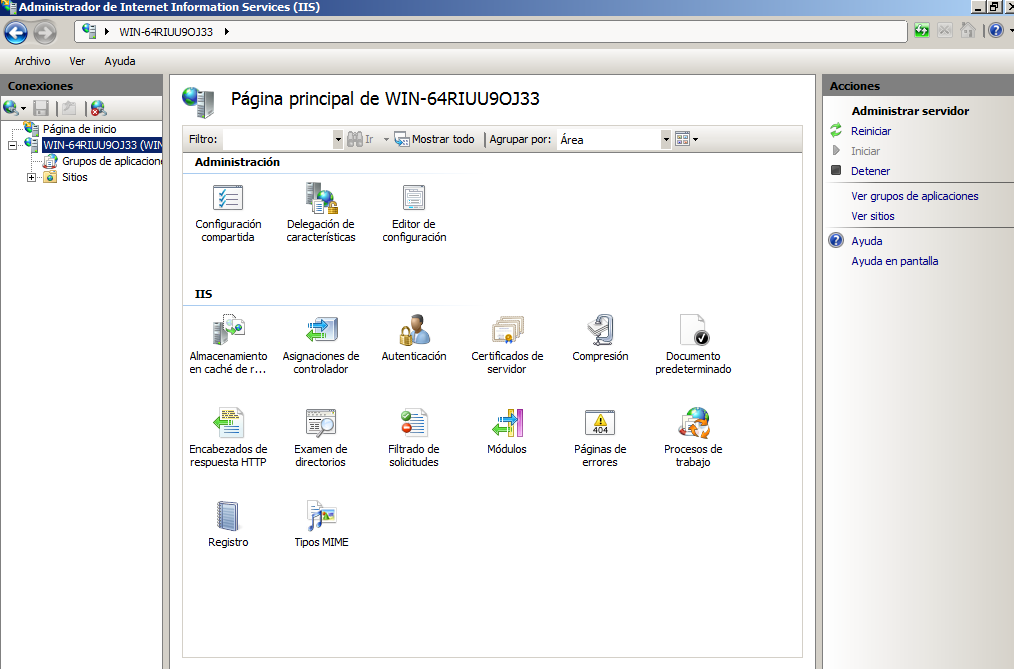
\includegraphics[width=1\textwidth]{c07f01}
	\caption{Consola de configuración de IIS.}
	\label{fig:c07f01}
\end{figure}

En la ventana central, nos aparecerán una serie de iconos agrupados por diferentes áreas. A nosotros nos interesará la área IIS, y dentro de ella el icono con el nombre "Compresión".

Podemos comprobar en nuestro caso que la compresión estática y dinámica está activada.

\begin{figure}[H]
	\centering
	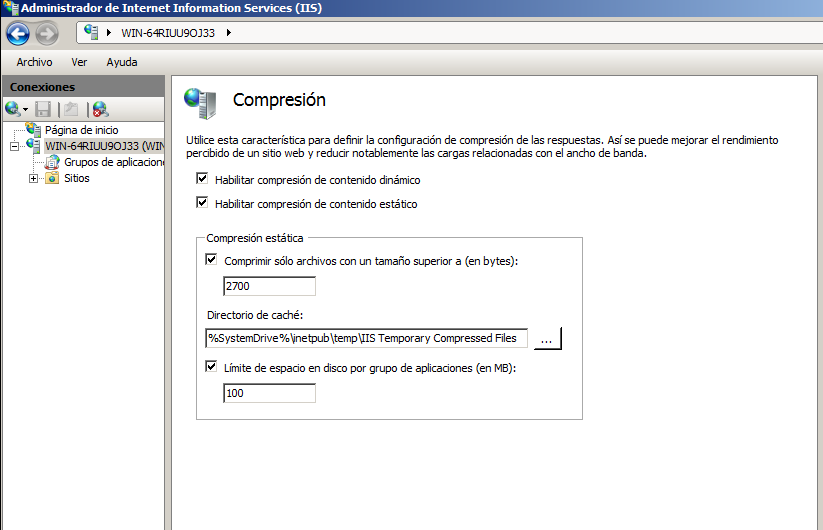
\includegraphics[width=1\textwidth]{c07f02}
	\caption{Configuración de la compresión de nuestro servidor.}
	\label{fig:c07f02}
\end{figure}

Ahora comprobaremos que funciona correctamente usando CURL:\\

Primero nos bajamos los binarios e instalamos\\

\begin{figure}[H]
	\centering
	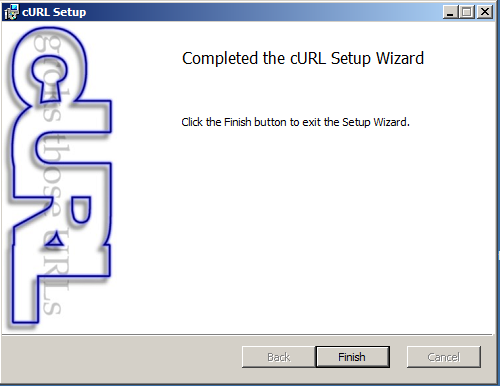
\includegraphics[width=1\textwidth]{c07f03}
	\caption{Instalación finalizada de CURL.}
	\label{fig:c07f03}
\end{figure}

\begin{figure}[H]
	\centering
	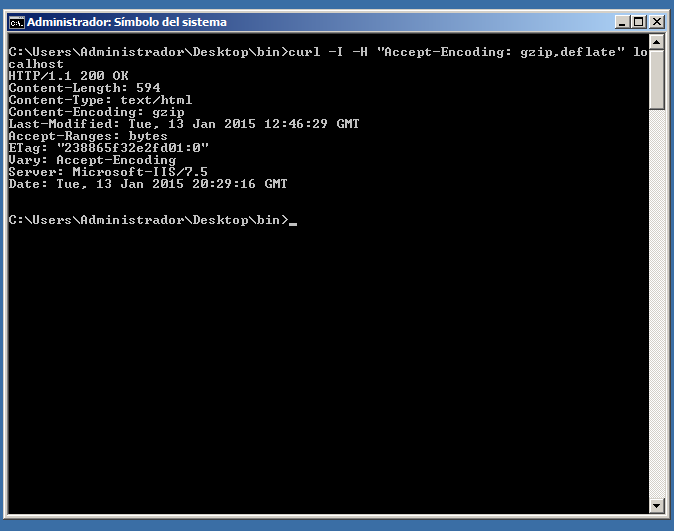
\includegraphics[width=1\textwidth]{c07f04}
	\caption{Comprobación del funcionamiento de la compresión por medio del comando CURL.}
	\label{fig:c07f04}
\end{figure}


\clearpage
%----------------------------------------------------------------------------------------
% CUESTION 8
%----------------------------------------------------------------------------------------
\section{Al igual que ha visto cómo se puede mejorar un servidor web (Práctica 5 Sección 3.1), elija un servicio (el que usted quiera) y modifique un parámetro para mejorar su comportamiento. (9.b) Monitorice el servicio antes y después de	la modificación del parámetro aplicando cargas al sistema (antes y después) mostrando los resultados de la monitorización.}

He decidido probar que sistema de RAID en Windows es más rápido. Para ello he usado mi benchmark que creé en la sesión anterior de practicas en el cual me daba la velocidad de escritura y lectura de disco en MB/s.\\

Posteriormente he ido cambiando la configuración de 2 discos de prueba virtuales alternando entre RAID0 y RAID1 y pasándole el test a cada una de las configuraciones obteniendo los siguientes resultados:

Para RAID0:
\begin{figure}[H]
	\centering
	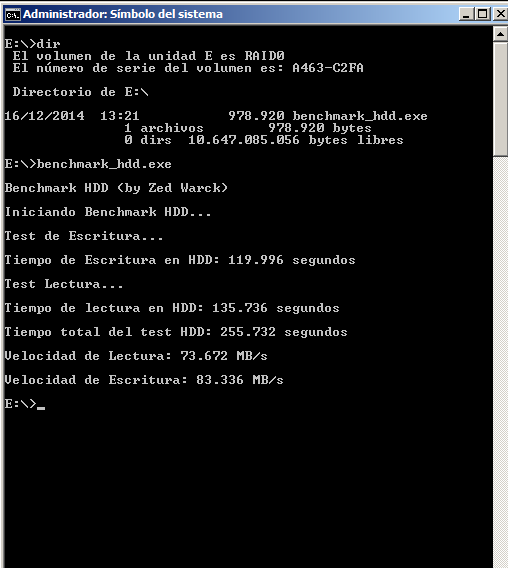
\includegraphics[width=0.5\textwidth]{c08f04}
	\caption{Benchmark para RAID0.}
	\label{fig:c08f04}
\end{figure}
\clearpage
Para RAID1:
\begin{figure}[H]
	\centering
	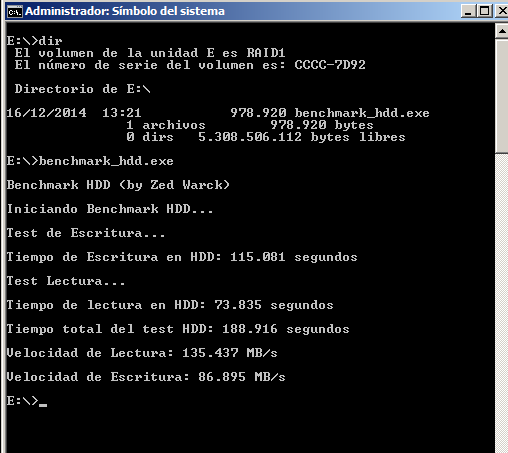
\includegraphics[width=0.7\textwidth]{c08f05}
	\caption{Benchmark para RAID1.}
	\label{fig:c08f05}
\end{figure}

Podemos observar que los accesos de escritora no varían demasiado, en cambio los de lectura si hay alguna gran diferencia, mejorando notablemente los tiempos de lectura para el sistema de RAID1 el más rápido.

\clearpage
%----------------------------------------------------------------------------------------
% CUESTION OPCIONAL 1
%----------------------------------------------------------------------------------------
\section{Instalación y configuración de un sistema KDC en Centos 6.5.}

Se ha instalado Centos 6.5 por motivos de compatibilidad con 2 interfaces de red, una para el sistema local y otra para la red externa.\\

Despues de la instalación Centos tiene desactivadas las interfaces de red por defecto, para ello editamos los archivos /etc/sysconfig/network-scripts/ifcfg-eth0 y /etc/sysconfig/network-scripts/ifcfg-eth1 y cambiamos la configuración colocando el valor ONBOOT="yes"  ademas ya que estamos es recomendable configurar las ips que sean estáticas, por lo tanto configuramos 2 subredes diferentes para cada una de las interfaces.




Despues instalamos NTP que nos hará falta para la sincronización temporal de las peticiones. Para ello:

yum -y install ntp ntpdate

y luego tenemos que abrir el puerto 123 UDP, para ello:

nano /etc/sysconfig/iptables

y añadimos: -A INPUT -m state --state NEW -m udp -p udp --dport 123 -j ACCEPT

posteriormente: service iptables restart






\clearpage
\bibliography{citas} %archivo citas.bib que contiene las entradas 
\bibliographystyle{unsrt} % hay varias formas de citar


\end{document}